\documentclass[xetex,colorlinks]{beamer} % Use XeTeX for direct UTF-8

\usepackage{fontspec} % Set fonts to UTF-8
\usepackage{listings} % Source code highlighting
\usepackage{adjustbox} % Resizing source code
\usepackage{hologo} % Nice logos, also for engines
\usepackage{qrcode} % QR code generator!
\usepackage{tikz} % Image generation
\usepackage{pstricks}
\usepackage[scaled=13]{CountriesOfEurope}
\usetheme{Singapore}
\usecolortheme{dove}
\hypersetup{allcolors=blue}

\title{Introduction to \hologo{LaTeXTeX}}
\subtitle{Workshop}
\author{Dainius Masiliūnas} % This requires XeTeX + fontspec; alternatively you can use \={u}
\institute{Laboratory of Geo-Information Science and Remote Sensing\\ Wageningen University \& Research}

\begin{document}
  \begin{frame}
    \titlepage
  \end{frame}

  \begin{frame}
    \frametitle{Table of contents}
    \tableofcontents
  \end{frame}

  \section{Theory}
  \subsection{Background}
  \subsubsection{Background}
  \begin{frame}
    \frametitle{Background}
    \begin{columns}
      \column{0.7\textwidth}
      \begin{itemize}
	\item Writing reports, papers, theses, articles, ...
	\item Office text processors: Microsoft Office Word, LibreOffice Writer, WPS Office Words, Calligra Words etc.
	\item Seemingly good software?
	\item But has irritations...
	\item Professionals use \TeX{}, a markup language for making documents
	\item Why?
      \end{itemize}
      \column{0.3\textwidth}
       % File folder with archived pages
% Author:	Leo Arnold
% Contact:	tex@arney.de
% License:	CC BY-SA 3.0
%\documentclass{article}
%\usepackage{tikz}
%\begin{document}

% Scale to your needs
\scalebox{0.1}{
  % All measures in centimeters
  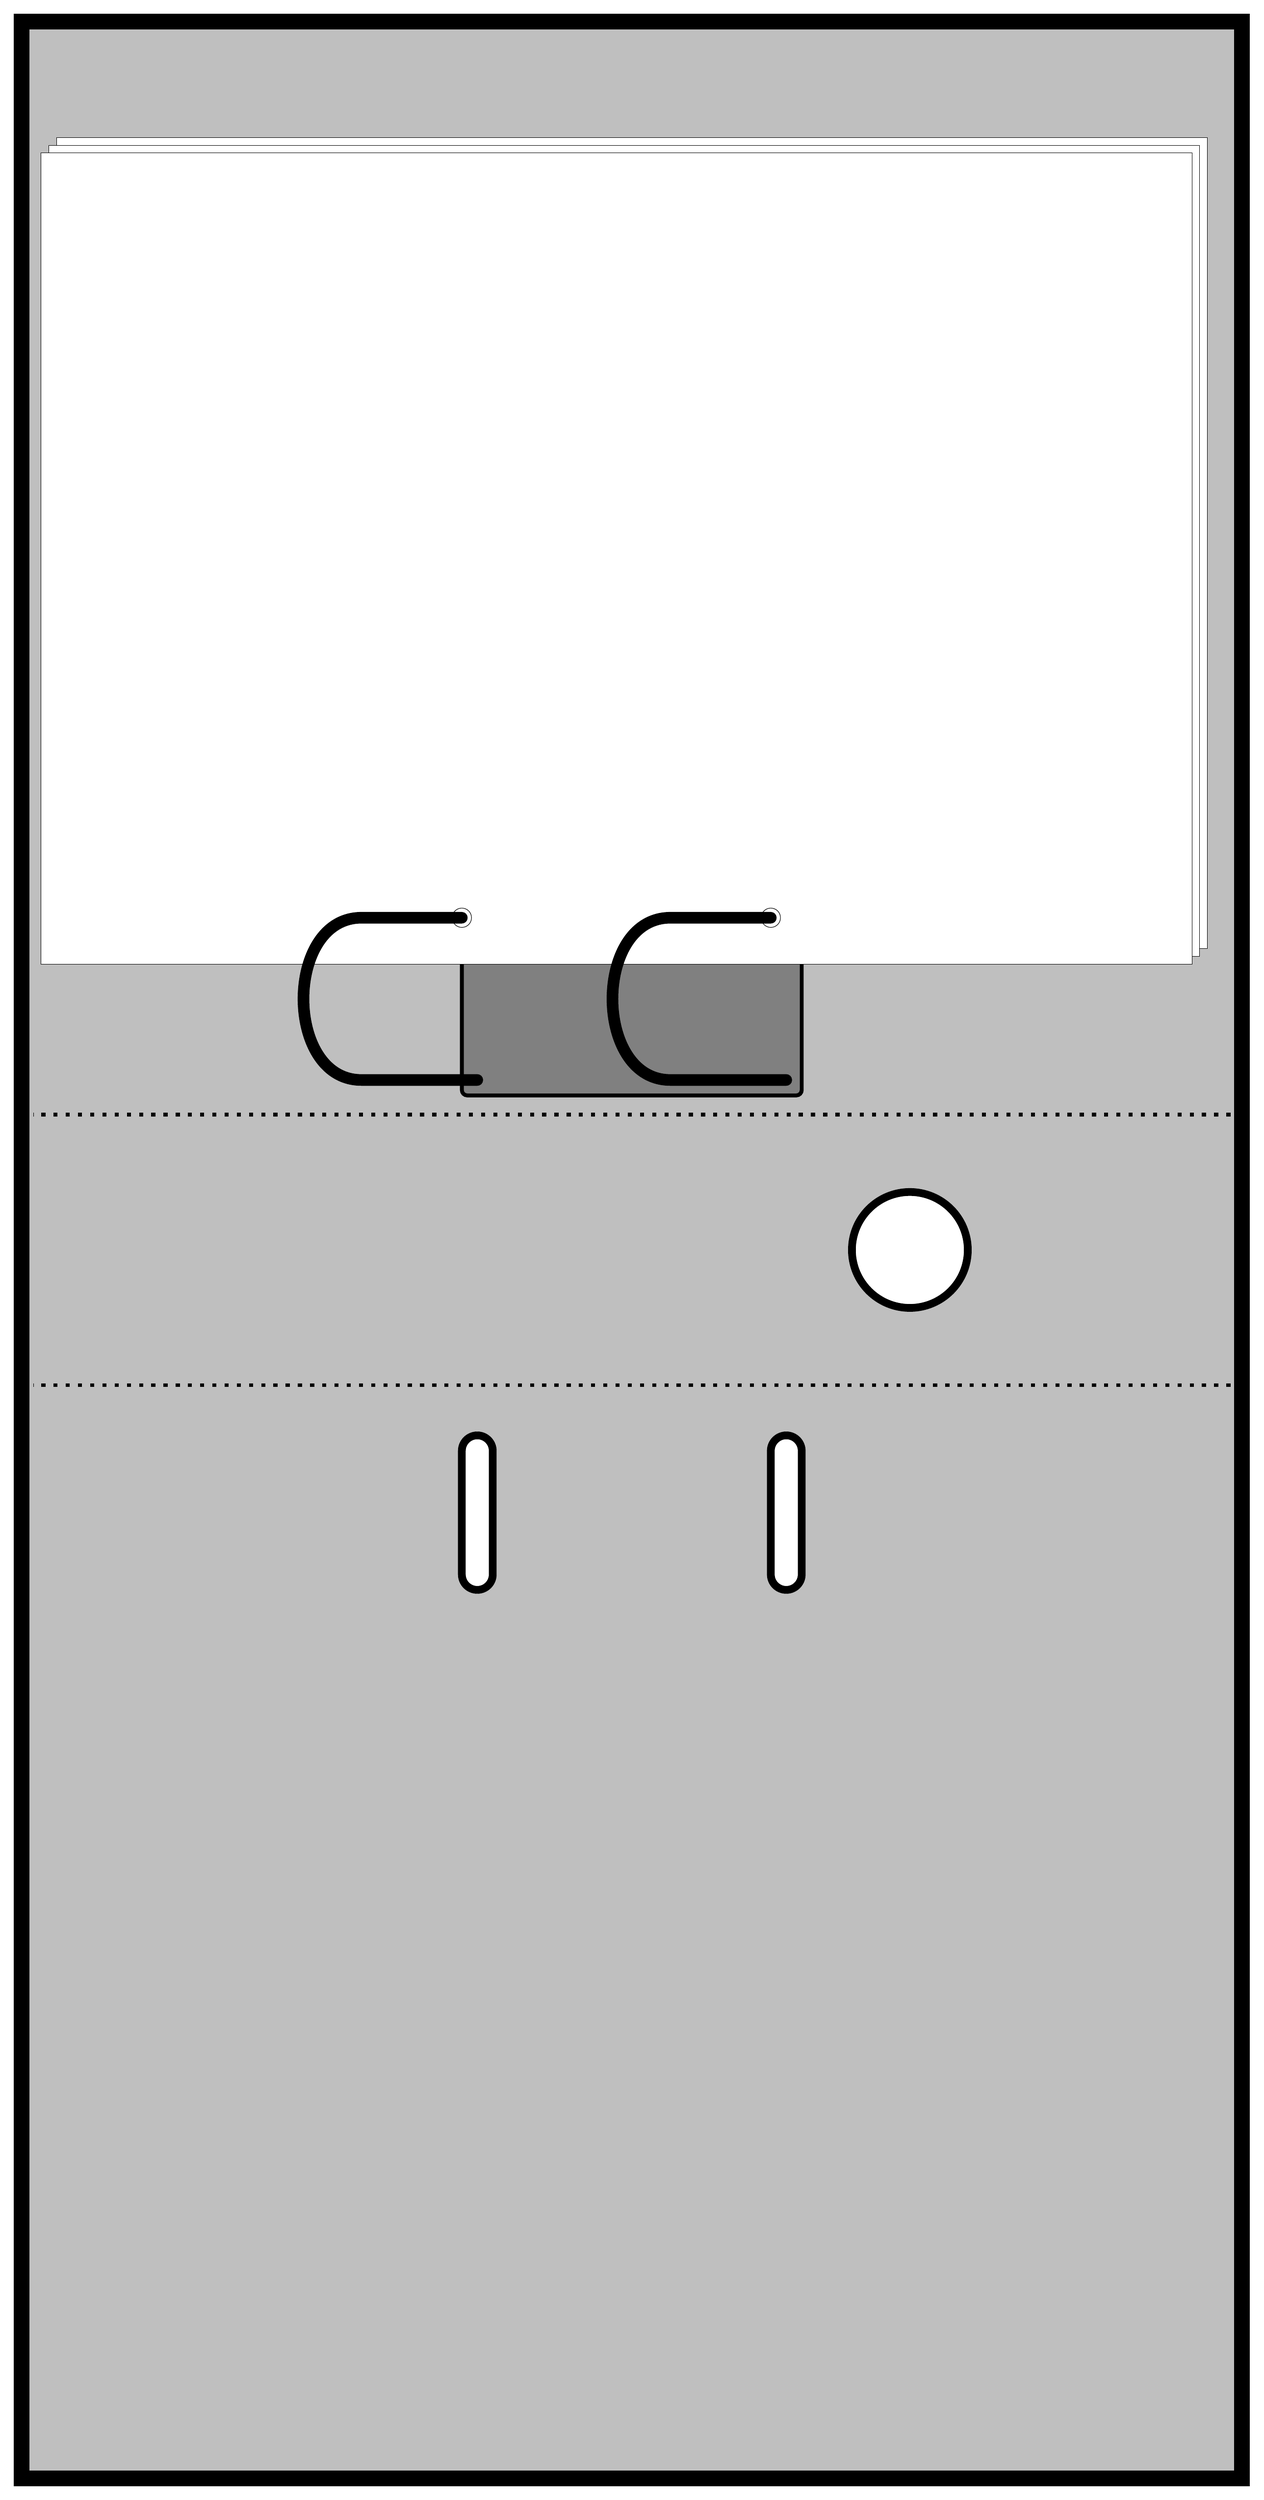
\begin{tikzpicture}[rotate=90]
    % Basic cardboard
    \draw[fill=black]
      (-32,0) rectangle (32,32);
    \draw[fill=gray!50]
      (-31.6,0.4) rectangle (31.6,31.6);

    % Fold lines
    \foreach \i in {-1, 1} {
      \draw[loosely dashed, line width=1mm]
        (\i*3.5,0.5) -- (\i*3.5,31.5);
    }

    % Finger hole
    \draw[fill=white, line width=2mm]
      (0,8.8) circle (1.5);

    % Metal plate
    \draw[fill=gray, line width=1mm, rounded corners]
      (4,11.6) rectangle (9,20.4);

    \foreach \i in {0, 1, 2} {
      % Filed pages
      \draw[fill=white, very thin, shift={(-\i*0.2,\i*0.2)}]
        (7.8,1.1) rectangle (28.8,30.9);
      % Punched holes
      \draw[fill=white, shift={(-\i*0.2,\i*0.2)}]
        (9,12) circle (0.25);
      \draw[fill=white, shift={(-\i*0.2,\i*0.2)}]
        (9,20) circle (0.25);
    }

    \foreach \i in {0, 1} {
      % Metal skewers
      \draw[line cap=round, line width=3mm, shift={(0,\i*8)}]
        (4.4,12) --
        (4.4,15) to [controls=+(90:2) and +(90:2)] (8.6,15)
         -- (8.6,12.4);
      % Holes opposite to skewers
      \draw[fill=white, line width=2mm, rounded corners=4mm, shift={(0,\i*8)}]
        (-8.8,11.6) rectangle (-4.8,12.4);
    }
  \end{tikzpicture}
}

%\end{document}

    \end{columns}
  \end{frame}
  
  \subsubsection{Issues with Office}
  \begin{frame}
    \frametitle{Issues with Office}
    \begin{columns}
      \column{0.85\textwidth}
      \begin{itemize}
      \item Images: they never stay in place, go above text, outside of caption boxes, etc.
      \item Copy-pasting text (or worse, tables) leads to formatting problems
      \item Different office programs render the same files differently
      \item Bibliography management is a hassle, citation styles are too rigid
      \item Math formulas handled by another program altogether
      \item Reformatting (for publishing etc.) is tricky
      \item Large documents/images become very slow
      \item \TeX{} solves that, and more: it's fun!
      \end{itemize}
      \column{0.15\textwidth}
      
\definecolor{c9cd1f1}{RGB}{156,209,241}
\definecolor{c625b6c}{RGB}{98,91,108}
\definecolor{c6d78b0}{RGB}{109,120,176}
\definecolor{cd0ceeb}{RGB}{208,206,235}
\definecolor{cd3d2d2}{RGB}{211,210,210}
\definecolor{cffffff}{RGB}{255,255,255}
\definecolor{c231f20}{RGB}{35,31,32}


\begin{tikzpicture}[y=0.80pt, x=0.80pt, yscale=-1.000000, xscale=1.000000, inner sep=0pt, outer sep=0pt]
\begin{scope}[cm={{1.25,0.0,0.0,-1.25,(-182.6425,164.14935)}}]
  \path[fill=c9cd1f1,even odd rule] (189.5860,81.5277) .. controls
    (188.3430,83.0125) and (185.5120,83.7723) .. (181.0230,83.7379) .. controls
    (176.5690,83.7031) and (171.7690,82.9434) .. (166.6590,81.4242) .. controls
    (161.5830,79.9395) and (157.6470,78.1094) .. (154.9190,75.9688) .. controls
    (152.1910,73.8277) and (151.4320,72.0324) .. (152.6750,70.5129) .. controls
    (153.9180,68.9938) and (156.7490,68.2340) .. (161.2380,68.3031) .. controls
    (165.7270,68.3031) and (170.4920,69.0973) .. (175.6020,70.5820) .. controls
    (180.7120,72.1016) and (184.6140,73.9316) .. (187.3410,76.0719) .. controls
    (190.0700,78.2129) and (190.8640,80.0086) .. (189.5860,81.5277);
  \path[fill=c9cd1f1,even odd rule] (185.7880,80.3883) .. controls
    (184.7870,81.5969) and (182.5420,82.1836) .. (178.9860,82.1496) .. controls
    (175.4290,82.1496) and (171.6310,81.5277) .. (167.5910,80.3195) .. controls
    (163.5520,79.1105) and (160.4440,77.6949) .. (158.2680,76.0035) .. controls
    (156.0930,74.2770) and (155.4720,72.8613) .. (156.4730,71.6523) .. controls
    (157.4740,70.4441) and (159.7190,69.8570) .. (163.2750,69.8918) .. controls
    (166.8320,69.8918) and (170.6300,70.5129) .. (174.6700,71.7215) .. controls
    (178.7440,72.9301) and (181.8170,74.3457) .. (183.9930,76.0719) .. controls
    (186.1680,77.7641) and (186.7890,79.1797) .. (185.7880,80.3883);
  \path[fill=c625b6c,even odd rule] (159.2360,126.4840) .. controls
    (159.9950,126.8980) and (160.8230,127.1060) .. (161.7210,127.1060) .. controls
    (162.6540,127.1400) and (163.4480,126.8980) .. (164.1040,126.4840) .. controls
    (164.8290,126.0360) and (165.2780,125.4140) .. (165.4850,124.6200) .. controls
    (165.8650,123.0320) and (165.9340,121.1670) .. (165.6920,119.0260) .. controls
    (165.0710,113.8810) and (164.6220,109.9100) .. (164.4490,107.1140) .. controls
    (164.1730,103.5570) and (163.8280,96.8242) .. (163.3790,86.9141) .. controls
    (163.3440,85.7746) and (162.9990,84.8426) .. (162.4460,84.1520) .. controls
    (161.8590,83.4961) and (161.2380,83.1508) .. (160.4780,83.1508) .. controls
    (159.6840,83.1160) and (159.0630,83.3578) .. (158.5450,83.9105) .. controls
    (157.9920,84.4973) and (157.6820,85.3605) .. (157.7160,86.5000) .. controls
    (157.7160,88.8824) and (157.8540,93.3363) .. (158.2000,99.8625) .. controls
    (158.0270,100.6570) and (157.4400,100.9680) .. (156.4730,100.7600) .. controls
    (155.9890,100.6570) and (155.6450,100.2770) .. (155.4720,99.6555) .. controls
    (155.1270,92.7840) and (154.9880,87.9500) .. (155.0570,85.2227) .. controls
    (155.0920,83.4270) and (155.6790,82.0109) .. (156.8530,81.0098) .. controls
    (157.9230,80.1121) and (159.2360,79.6977) .. (160.7200,79.7668) .. controls
    (162.2050,79.8703) and (163.4820,80.3883) .. (164.5530,81.3551) .. controls
    (165.7270,82.4602) and (166.3480,83.9105) .. (166.4180,85.6715) .. controls
    (166.6240,91.8520) and (167.0740,97.7219) .. (167.7980,103.3840) --
    (169.6280,118.6810) .. controls (170.0770,123.9980) and (169.0760,127.6580) ..
    (166.5900,129.5920) .. controls (165.0360,130.7660) and (163.2410,131.3530) ..
    (161.1690,131.3180) .. controls (158.9940,131.2840) and (157.1640,130.5930) ..
    (155.6790,129.2460) .. controls (153.8840,127.6240) and (152.8470,125.3790) ..
    (152.5370,122.4790) .. controls (151.2590,109.7380) and (150.7410,94.8211) ..
    (150.9480,77.6949) .. controls (151.0170,74.5875) and (152.0540,72.2395) ..
    (154.1590,70.6168) .. controls (156.0240,69.2355) and (158.3030,68.5793) ..
    (160.9960,68.8211) .. controls (163.6890,69.0285) and (165.9680,69.9609) ..
    (167.8330,71.6184) .. controls (169.9390,73.3789) and (170.9750,75.6234) ..
    (171.0090,78.2477) -- (171.3550,91.5414) .. controls (171.4240,93.5781) and
    (172.6670,95.9605) .. (175.1190,98.7230) .. controls (175.1190,99.3445) and
    (174.8770,99.8281) .. (174.4280,100.1730) .. controls (174.0480,100.5180) and
    (173.4960,100.6570) .. (172.8740,100.6910) .. controls (169.8360,97.6180) and
    (168.2820,94.8902) .. (168.3170,92.5082) -- (168.0400,78.5930) .. controls
    (167.9020,76.7285) and (167.1080,75.2090) .. (165.7270,74.1387) .. controls
    (164.4840,73.1719) and (162.9990,72.6539) .. (161.2040,72.6195) .. controls
    (159.4770,72.5848) and (157.9920,72.9992) .. (156.6800,73.9316) .. controls
    (155.2640,74.8637) and (154.5050,76.2797) .. (154.3670,78.0402) .. controls
    (154.0560,81.5277) and (154.1590,87.9848) .. (154.7120,97.4453) --
    (156.2660,120.0960) .. controls (156.4380,121.9960) and (156.8180,123.5150) ..
    (157.3710,124.6540) .. controls (157.7510,125.4140) and (158.3720,126.0360) ..
    (159.2360,126.4840);
  \path[fill=c6d78b0,even odd rule] (157.8540,126.3460) .. controls
    (159.0630,127.5890) and (160.5480,128.1410) .. (162.3770,128.0040) .. controls
    (164.2420,127.8310) and (165.6230,127.0020) .. (166.5550,125.5170) .. controls
    (167.0390,124.7580) and (167.3500,123.8250) .. (167.4190,122.6170) .. controls
    (167.4530,121.7540) and (167.4190,120.4070) .. (167.2460,118.6460) --
    (165.9680,105.8360) .. controls (165.5200,100.6220) and (165.1750,94.2344) ..
    (164.9330,86.7074) .. controls (164.8980,85.4988) and (164.4840,84.5313) ..
    (163.6890,83.8070) .. controls (162.9990,83.1508) and (162.1360,82.7707) ..
    (161.1000,82.7016) .. controls (160.1330,82.5980) and (159.2360,82.7707) ..
    (158.5450,83.2887) .. controls (157.7510,83.8070) and (157.3710,84.5313) ..
    (157.3360,85.5328) .. controls (157.3020,90.0219) and (157.4050,94.5449) ..
    (157.6470,99.1371) .. controls (158.0270,99.4137) and (158.0960,99.7246) ..
    (157.8890,100.0700) .. controls (157.6470,100.4150) and (157.3020,100.5530) ..
    (156.8180,100.5530) .. controls (156.2660,100.5530) and (155.9200,100.2770) ..
    (155.7820,99.7934) .. controls (155.6100,99.2754) and (155.8860,99.0340) ..
    (156.5420,98.9645) .. controls (156.2660,92.1281) and (156.1280,87.5012) ..
    (156.1970,85.0152) .. controls (156.1970,83.8070) and (156.7150,82.8746) ..
    (157.6820,82.2527) .. controls (158.5450,81.6660) and (159.6500,81.4590) ..
    (160.9270,81.5625) .. controls (162.2050,81.6660) and (163.2750,82.1145) ..
    (164.2070,82.8398) .. controls (165.2090,83.6688) and (165.7610,84.7039) ..
    (165.8650,86.0168) .. controls (166.3830,94.6832) and (166.7630,100.6220) ..
    (167.0390,103.7300) .. controls (167.4190,107.6660) and (168.0050,112.2240) ..
    (168.7650,117.4720) .. controls (169.4210,121.7540) and (169.0410,124.9990) ..
    (167.5220,127.2440) .. controls (166.1070,129.3160) and (164.1390,130.3170) ..
    (161.6870,130.2820) .. controls (159.1660,130.2480) and (157.1640,129.1430) ..
    (155.6790,126.9680) .. controls (154.9540,125.9320) and (154.4360,123.9290) ..
    (154.0210,121.0630) .. controls (152.7090,111.0500) and (152.1570,96.4441) ..
    (152.2950,77.2809) .. controls (152.2950,74.8637) and (153.2270,73.0340) ..
    (155.0920,71.7559) .. controls (156.7490,70.5820) and (158.8210,70.0297) ..
    (161.2720,70.1336) .. controls (163.6890,70.2715) and (165.7270,70.9621) ..
    (167.4530,72.3086) .. controls (169.3860,73.7590) and (170.3540,75.6582) ..
    (170.4230,78.0059) -- (170.7680,91.8520) .. controls (170.7680,94.2000) and
    (172.1490,96.6168) .. (174.8430,99.0684) .. controls (174.9800,99.2754) and
    (174.9460,99.5172) .. (174.7040,99.7934) .. controls (174.3590,100.1040) and
    (174.1520,100.2770) .. (174.0140,100.2430) .. controls (171.0790,97.0313) and
    (169.5940,94.2344) .. (169.5940,91.9555) .. controls (169.5940,83.1160) and
    (169.4910,78.3855) .. (169.2830,77.7297) .. controls (168.6960,75.6926) and
    (167.5570,74.1387) .. (165.8650,73.1027) .. controls (164.3800,72.2051) and
    (162.6880,71.7559) .. (160.8230,71.8250) .. controls (158.9940,71.8941) and
    (157.4050,72.4121) .. (156.0590,73.3445) .. controls (154.6770,74.3805) and
    (153.9180,75.6926) .. (153.8140,77.2809) .. controls (153.5380,81.1824) and
    (153.6070,87.7430) .. (154.0210,96.9617) .. controls (154.4360,105.8360) and
    (155.0230,113.7780) .. (155.7140,120.7180) .. controls (156.0240,123.2730) and
    (156.7150,125.1720) .. (157.8540,126.3460);
  \path[fill=cd0ceeb,even odd rule] (169.8700,78.4547) .. controls
    (169.7320,78.4203) and (169.6280,78.3512) .. (169.5600,78.1438) --
    (169.4550,77.4879) .. controls (168.9040,75.4508) and (167.7640,73.8969) ..
    (166.0720,72.8266) .. controls (164.5880,71.8941) and (162.8260,71.4797) ..
    (160.8930,71.5492) .. controls (159.0280,71.6184) and (157.4050,72.1703) ..
    (156.0590,73.1027) .. controls (154.6080,74.1387) and (153.7800,75.4508) ..
    (153.6420,77.0043) .. controls (153.6420,77.4188) and (153.5380,77.5574) ..
    (153.2620,77.5574) .. controls (152.9160,77.5223) and (152.8130,77.3152) ..
    (152.9510,76.9008) .. controls (153.2960,74.7598) and (154.3320,73.1027) ..
    (156.0590,71.9633) .. controls (157.6470,70.9621) and (159.4770,70.4785) ..
    (161.5830,70.6168) .. controls (163.6890,70.7203) and (165.5200,71.3418) ..
    (167.1080,72.5504) .. controls (168.8000,73.8277) and (169.8360,75.5539) ..
    (170.1810,77.6949) .. controls (170.2840,78.2129) and (170.1810,78.4891) ..
    (169.8700,78.4547);
  \path[fill=cd0ceeb,even odd rule] (157.5780,99.0340) -- (157.0600,98.8957) --
    (156.7840,93.3363) .. controls (156.6110,89.7801) and (156.5070,87.1902) ..
    (156.5420,85.5676) .. controls (156.5770,84.3590) and (157.0250,83.4270) ..
    (157.9230,82.7707) .. controls (158.7520,82.1496) and (159.7540,81.9078) ..
    (160.9270,81.9770) .. controls (162.1010,82.0461) and (163.1370,82.4602) ..
    (164.0350,83.1508) .. controls (165.0020,83.9797) and (165.5540,85.0152) ..
    (165.6920,86.3617) .. controls (165.7270,86.7418) and (165.6920,86.9141) ..
    (165.5200,86.9141) .. controls (165.3130,86.9141) and (165.2780,86.7074) ..
    (165.2780,86.3617) .. controls (165.1050,85.1188) and (164.5530,84.1520) ..
    (163.6890,83.3926) .. controls (162.8950,82.7367) and (161.9630,82.3563) ..
    (160.9270,82.3223) .. controls (159.8910,82.2871) and (159.0280,82.5641) ..
    (158.3370,83.1508) .. controls (157.5780,83.8410) and (157.1980,84.7730) ..
    (157.1980,86.0168) -- (157.5780,99.0340);
  \path[fill=cd0ceeb,even odd rule] (158.8900,128.0380) .. controls
    (160.4090,129.0740) and (161.9630,129.4880) .. (163.6550,129.2460) .. controls
    (165.4160,128.9700) and (166.6930,128.0730) .. (167.4530,126.5190) .. controls
    (168.1090,125.3110) and (168.3850,123.9290) .. (168.3850,122.3410) .. controls
    (168.3510,122.0300) and (168.4200,121.8570) .. (168.6620,121.8230) .. controls
    (168.8340,121.7880) and (168.9380,121.9960) .. (168.9380,122.4450) .. controls
    (168.9380,124.2750) and (168.5590,125.8970) .. (167.6950,127.3480) .. controls
    (166.7970,128.8320) and (165.4850,129.7300) .. (163.6550,130.0060) .. controls
    (161.8590,130.3170) and (160.0980,129.9020) .. (158.4410,128.8320) .. controls
    (158.2000,128.5910) and (158.1300,128.3490) .. (158.2680,128.1410) .. controls
    (158.4410,127.9000) and (158.6480,127.8650) .. (158.8900,128.0380);
  \path[fill=c625b6c,even odd rule] (147.1500,109.5300) .. controls
    (146.9090,107.8390) and (147.3230,106.3540) .. (148.2890,105.0070) .. controls
    (149.2910,103.6610) and (150.6380,102.9010) .. (152.2950,102.6590) .. controls
    (153.9870,102.4180) and (155.4720,102.7970) .. (156.8180,103.7990) .. controls
    (158.1650,104.8000) and (158.9240,106.1120) .. (159.1660,107.8040) .. controls
    (159.4080,109.4620) and (159.0280,110.9460) .. (158.0270,112.2930) .. controls
    (157.0250,113.6050) and (155.6790,114.4340) .. (154.0210,114.6410) .. controls
    (152.3640,114.9170) and (150.8790,114.5030) .. (149.5330,113.5360) .. controls
    (148.1860,112.5000) and (147.3920,111.1880) .. (147.1500,109.5300);
  \path[fill=cd3d2d2,even odd rule] (149.3950,112.5000) .. controls
    (148.0830,111.7750) and (147.3570,110.7740) .. (147.1500,109.5300) .. controls
    (146.9780,108.2190) and (147.3920,106.9750) .. (148.4280,105.7670) .. controls
    (149.4980,104.4890) and (150.8100,103.7300) .. (152.4330,103.4880) .. controls
    (154.0560,103.2460) and (155.5410,103.5910) .. (156.9220,104.5240) .. controls
    (158.2340,105.4210) and (158.9940,106.4920) .. (159.1660,107.8040) .. controls
    (159.3390,109.0470) and (158.9240,110.2210) .. (157.8540,111.2570) .. controls
    (156.8180,112.2930) and (155.4720,112.9840) .. (153.8140,113.1910) .. controls
    (152.1570,113.4320) and (150.6720,113.1910) .. (149.3950,112.5000);
  \path[fill=cffffff,even odd rule] (153.6420,112.1550) .. controls
    (152.0880,112.3960) and (150.7070,112.2240) .. (149.4980,111.7060) .. controls
    (148.2890,111.1880) and (147.5990,110.4630) .. (147.4610,109.4620) .. controls
    (147.3230,108.4250) and (147.7380,107.4590) .. (148.7390,106.4580) .. controls
    (149.7750,105.3870) and (151.0520,104.7310) .. (152.5710,104.5240) .. controls
    (154.0900,104.3170) and (155.4720,104.5590) .. (156.7840,105.2840) .. controls
    (157.9920,105.9740) and (158.6820,106.8030) .. (158.8550,107.8390) .. controls
    (158.9940,108.8400) and (158.5450,109.7380) .. (157.5090,110.5660) .. controls
    (156.5070,111.3950) and (155.2300,111.9480) .. (153.6420,112.1550);
  \path[fill=c231f20,even odd rule] (153.4000,110.4630) .. controls
    (152.8470,110.4970) and (152.2950,110.3940) .. (151.8460,110.0490) .. controls
    (151.3970,109.7030) and (151.1210,109.2200) .. (151.0170,108.6330) .. controls
    (150.9480,108.0460) and (151.0860,107.5280) .. (151.4320,107.0790) .. controls
    (151.7770,106.5960) and (152.2610,106.3540) .. (152.8470,106.2500) .. controls
    (153.4000,106.1810) and (153.9180,106.3200) .. (154.4010,106.6650) .. controls
    (154.8850,107.0100) and (155.1270,107.4930) .. (155.2300,108.0460) .. controls
    (155.2990,108.5980) and (155.1610,109.1160) .. (154.8160,109.6340) .. controls
    (154.4710,110.0830) and (153.9870,110.3590) .. (153.4000,110.4630);
  \path[fill=c625b6c,even odd rule] (168.0050,115.3310) .. controls
    (166.3140,115.5730) and (164.8290,115.1590) .. (163.5170,114.1920) .. controls
    (162.2050,113.1910) and (161.4110,111.8440) .. (161.1690,110.1520) .. controls
    (160.9270,108.5290) and (161.3070,107.0100) .. (162.3080,105.6630) .. controls
    (163.3100,104.3170) and (164.6220,103.5570) .. (166.3140,103.3150) .. controls
    (167.9710,103.0740) and (169.4550,103.4540) .. (170.8020,104.4550) .. controls
    (172.1490,105.4560) and (172.9430,106.8030) .. (173.1500,108.4250) .. controls
    (173.3920,110.1180) and (173.0470,111.6020) .. (172.0110,112.9840) .. controls
    (171.0090,114.2960) and (169.6630,115.0900) .. (168.0050,115.3310);
  \path[fill=cd3d2d2,even odd rule] (167.7980,113.8810) .. controls
    (166.1410,114.1230) and (164.6570,113.8470) .. (163.3440,113.1210) .. controls
    (162.0670,112.3960) and (161.3410,111.4300) .. (161.1690,110.1520) .. controls
    (160.9620,108.8750) and (161.3760,107.5970) .. (162.4120,106.3890) .. controls
    (163.4480,105.1110) and (164.8290,104.3860) .. (166.4180,104.1790) .. controls
    (168.0400,103.9370) and (169.5250,104.2820) .. (170.9060,105.2140) .. controls
    (172.2180,106.0780) and (172.9780,107.1480) .. (173.1500,108.4250) .. controls
    (173.3570,109.7030) and (172.9090,110.8430) .. (171.8730,111.9480) .. controls
    (170.8370,112.9840) and (169.4910,113.6050) .. (167.7980,113.8810);
  \path[fill=cffffff,even odd rule] (161.5490,110.1180) .. controls
    (161.4110,109.1160) and (161.8250,108.1150) .. (162.7920,107.1480) .. controls
    (163.8280,106.1120) and (165.0710,105.4560) .. (166.5550,105.2490) .. controls
    (168.0750,105.0420) and (169.4550,105.2840) .. (170.7340,106.0090) .. controls
    (171.9080,106.6650) and (172.5980,107.4930) .. (172.7360,108.5290) .. controls
    (172.8740,109.4620) and (172.4600,110.3590) .. (171.4580,111.1880) .. controls
    (170.4570,112.0170) and (169.1800,112.5350) .. (167.6610,112.7420) .. controls
    (166.0720,112.9840) and (164.7250,112.8450) .. (163.5520,112.2930) .. controls
    (162.3430,111.8090) and (161.6870,111.0500) .. (161.5490,110.1180);
  \path[fill=c231f20,even odd rule] (169.2140,108.7020) .. controls
    (169.2830,109.2890) and (169.1800,109.8070) .. (168.8340,110.2900) .. controls
    (168.4890,110.7390) and (168.0050,111.0150) .. (167.4190,111.1190) .. controls
    (166.8320,111.1880) and (166.3140,111.0500) .. (165.8650,110.7050) .. controls
    (165.3810,110.3590) and (165.0710,109.8760) .. (165.0020,109.2890) .. controls
    (164.9330,108.7360) and (165.0710,108.1840) .. (165.4160,107.7350) .. controls
    (165.7610,107.2520) and (166.2450,106.9750) .. (166.7970,106.8720) .. controls
    (167.3840,106.8030) and (167.9020,106.9410) .. (168.3850,107.2860) .. controls
    (168.8680,107.6320) and (169.1450,108.1150) .. (169.2140,108.7020);
  \path[fill=c231f20,even odd rule] (151.5360,122.3410) .. controls
    (149.2220,121.5120) and (147.4260,119.4750) .. (146.1140,116.1600) .. controls
    (148.8420,118.9230) and (151.0520,120.1660) .. (152.8470,119.8890) --
    (151.5360,122.3410);
  \path[fill=c231f20,even odd rule] (168.3850,121.3050) -- (167.4530,118.6460) ..
    controls (168.7310,118.6120) and (170.1810,118.1630) .. (171.8380,117.3340) ..
    controls (173.4610,116.5050) and (174.9800,115.4000) .. (176.4650,114.0540) ..
    controls (174.2550,117.5760) and (171.5620,119.9930) .. (168.3850,121.3050);
\end{scope}

\end{tikzpicture}


    \end{columns}
  \end{frame}
  
  \subsubsection{\TeX{} history and example}
  \begin{frame}
    \frametitle{\TeX{}}
    \begin{columns}
    \column{0.94\textwidth}
    \begin{itemize}
     \item A typesetting system made in 1978 (MS Word: 1990)
     \begin{itemize}
      \item \LaTeX{} (1984): additions to base \TeX{} for ease of use
      \item \hologo{ConTeXt} (1996, Dutch): additions to \TeX{} for more control
     \end{itemize}
     \item Document files are plain text (\texttt{.tex}, source code, markup)
     \item An engine (compiler) is used to turn it into a standard read-only document (PDF, PS)
     \begin{itemize}
      \item \hologo{pdfLaTeX}
      \item \hologo{XeTeX}
     \end{itemize}
     \item Highly extensible, heavily package-oriented: ``there's a package for that''
     \item Available as a distribution: collection of engines and packages
     \item Free and open-source software, cross-platform
    \end{itemize}
    \column{0.06\textwidth}
    
\definecolor{c100069}{RGB}{16,0,105}
\definecolor{cffffff}{RGB}{255,255,255}


\begin{tikzpicture}[y=0.80pt, x=0.80pt, yscale=-0.1000000, xscale=0.1000000, inner sep=0pt, outer sep=0pt]
\path[fill=c100069] (408.0000,204.0000) .. controls (408.0000,149.8940) and
  (386.5040,98.0090) .. (348.2470,59.7530) .. controls (309.9910,21.4970) and
  (258.1070,0.0000) .. (204.0000,0.0000) .. controls (149.8940,0.0000) and
  (98.0090,21.4970) .. (59.7530,59.7530) .. controls (21.4980,98.0100) and
  (0.0000,149.8940) .. (0.0000,204.0000) .. controls (0.0000,258.1070) and
  (21.4970,309.9910) .. (59.7530,348.2470) .. controls (98.0090,386.5040) and
  (149.8940,408.0000) .. (204.0000,408.0000) .. controls (258.1070,408.0000) and
  (309.9910,386.5040) .. (348.2470,348.2470) .. controls (386.5040,309.9910) and
  (408.0000,258.1070) .. (408.0000,204.0000) -- cycle;
\begin{scope}[shift={(-0.397,-0.396)}]
  \path[fill=cffffff] (115.3830,132.4490) .. controls (114.2210,127.4130) and
    (113.1880,124.9600) .. (111.1220,122.3780) .. controls (107.5070,117.8590) and
    (101.9550,115.5350) .. (95.2410,115.5350) .. controls (80.0050,115.5350) and
    (70.8370,127.9310) .. (70.8370,148.7190) .. controls (70.8370,169.2490) and
    (79.6170,181.3860) .. (94.5950,181.3860) .. controls (106.6030,181.3860) and
    (114.2210,174.5430) .. (115.3840,162.5340) -- (134.2360,162.5340) .. controls
    (133.0740,184.0970) and (117.4500,197.6550) .. (94.0800,197.6550) .. controls
    (67.8690,197.6550) and (51.4700,178.6750) .. (51.4700,148.4600) .. controls
    (51.4700,117.9880) and (67.9970,99.0070) .. (94.5960,99.0070) .. controls
    (108.6700,99.0070) and (120.2910,104.3010) .. (127.5220,113.8560) .. controls
    (131.5240,119.1500) and (133.2030,124.3150) .. (133.8490,132.4490) --
    (115.3830,132.4490) -- cycle;
\end{scope}
\begin{scope}[shift={(-0.397,-0.396)}]
  \path[fill=cffffff] (236.8080,56.0480) .. controls (245.2010,65.0870) and
    (249.9780,78.2560) .. (249.9780,92.9760) .. controls (249.9780,106.2750) and
    (244.9430,119.9620) .. (236.8080,128.6130) .. controls (228.6730,137.3930) and
    (218.0850,141.6540) .. (204.6570,141.6540) .. controls (191.2290,141.6540) and
    (180.6410,137.3930) .. (172.5060,128.6130) .. controls (164.1130,119.7040) and
    (159.3360,106.4050) .. (159.3360,92.3300) .. controls (159.3360,78.2550) and
    (164.1130,65.0860) .. (172.5060,56.0470) .. controls (180.5110,47.3960) and
    (191.3580,43.0060) .. (204.5280,43.0060) .. controls (218.0850,43.0070) and
    (228.5440,47.1390) .. (236.8080,56.0480) -- cycle(178.7040,92.3310) ..
    controls (178.7040,112.0860) and (189.0340,125.1270) .. (204.6570,125.1270) ..
    controls (220.1520,125.1270) and (230.6110,112.0860) .. (230.6110,92.8470) ..
    controls (230.6110,72.4460) and (220.5390,59.5340) .. (204.6570,59.5340) ..
    controls (189.0340,59.5350) and (178.7040,72.5760) .. (178.7040,92.3310) --
    cycle;
\end{scope}
\begin{scope}[shift={(-0.397,-0.396)}]
  \path[fill=cffffff] (297.9330,129.0270) -- (297.9330,194.1030) --
    (278.5650,194.1030) -- (278.5650,99.9750) -- (298.4500,99.9750) --
    (335.7650,164.0180) -- (335.7650,99.9750) -- (355.1330,99.9750) --
    (355.1330,194.1030) -- (335.7650,194.1030) -- (297.9330,129.0270) -- cycle;
\end{scope}
\begin{scope}[shift={(-0.397,-0.396)}]
  \path[fill=cffffff] (102.6650,306.1020) -- (83.2970,306.1020) --
    (83.2970,228.1140) -- (54.7610,228.1140) -- (54.7610,211.9740) --
    (130.1670,211.9740) -- (130.1670,228.1140) -- (102.6640,228.1140) --
    (102.6640,306.1020) -- cycle;
\end{scope}
\begin{scope}[shift={(-0.397,-0.396)}]
  \path[fill=cffffff] (190.9060,233.9620) -- (241.9080,233.9620) --
    (241.9080,250.1020) -- (171.5380,250.1020) -- (171.5380,155.9740) --
    (239.5840,155.9740) -- (239.5840,172.1140) -- (190.9050,172.1140) --
    (190.9050,193.4190) -- (235.9680,193.4190) -- (235.9680,209.5590) --
    (190.9050,209.5590) -- (190.9050,233.9620) -- cycle;
\end{scope}
\begin{scope}[shift={(-0.397,-0.396)}]
  \path[fill=cffffff] (357.6520,306.1020) -- (334.6690,306.1020) --
    (316.5920,273.4350) -- (298.6450,306.1020) -- (276.1780,306.1020) --
    (305.8750,258.7150) -- (277.2110,211.9740) -- (300.1930,211.9740) --
    (316.7200,242.9620) -- (334.0230,211.9740) -- (356.4900,211.9740) --
    (327.4380,258.0700) -- (357.6520,306.1020) -- cycle;
\end{scope}
\begin{scope}[shift={(-0.397,-0.396)}]
  \path[fill=cffffff] (214.6640,362.1010) -- (195.2960,362.1010) --
    (195.2960,284.1130) -- (166.7600,284.1130) -- (166.7600,267.9730) --
    (242.1660,267.9730) -- (242.1660,284.1130) -- (214.6640,284.1130) --
    (214.6640,362.1010) -- cycle;
\end{scope}
\path[draw=cffffff,line join=round,miter limit=10.00,rounded corners=0.0000cm]
  (36.0000,92.0000) rectangle (148.0000,204.0000);
\path[draw=cffffff,line join=round,miter limit=10.00,rounded corners=0.0000cm]
  (148.0000,36.0000) rectangle (260.0000,148.0000);
\path[draw=cffffff,line join=round,miter limit=10.00,rounded corners=0.0000cm]
  (260.0000,92.0000) rectangle (372.0000,204.0000);
\path[draw=cffffff,line join=round,miter limit=10.00,rounded corners=0.0000cm]
  (36.0000,204.0000) rectangle (148.0000,316.0000);
\path[draw=cffffff,line join=round,miter limit=10.00,rounded corners=0.0000cm]
  (148.0000,148.0000) rectangle (260.0000,260.0000);
\path[draw=cffffff,line join=round,miter limit=10.00,rounded corners=0.0000cm]
  (260.0000,204.0000) rectangle (372.0000,316.0000);
\path[draw=cffffff,line join=round,miter limit=10.00,rounded corners=0.0000cm]
  (148.0000,260.0000) rectangle (260.0000,372.0000);

\end{tikzpicture}


    %LaTeX with PSTricks extensions
%%Creator: inkscape 0.92.4
%%Please note this file requires PSTricks extensions
\psset{xunit=.035pt,yunit=.035pt,runit=.035pt}
\begin{pspicture}(900,600)
{
\newrgbcolor{curcolor}{0.12941177 0.27450982 0.54509807}
\pscustom[linestyle=none,fillstyle=solid,fillcolor=curcolor]
{
\newpath
\moveto(0,600)
\lineto(900,600)
\lineto(900,0)
\lineto(0,0)
\closepath
}
}
{
\newrgbcolor{curcolor}{1 1 1}
\pscustom[linestyle=none,fillstyle=solid,fillcolor=curcolor]
{
\newpath
\moveto(0,600)
\lineto(900,600)
\lineto(900,200)
\lineto(0,200)
\closepath
}
}
{
\newrgbcolor{curcolor}{0.68235296 0.10980392 0.15686275}
\pscustom[linestyle=none,fillstyle=solid,fillcolor=curcolor]
{
\newpath
\moveto(0,600)
\lineto(900,600)
\lineto(900,400)
\lineto(0,400)
\closepath
}
}
\end{pspicture}

    % For some reason below no longer works with TeXLive 2018 (or I'm missing some package), XeLaTeX just crashes
    %\CountriesOfEuropeFamily{}
    %\Netherlands{}
    \end{columns}
  \end{frame}
  
  \begin{frame}
    \frametitle{Example}
    \begin{columns}[c]
      \column{.4\textwidth}
      \begin{adjustbox}{width=\textwidth,height=\textheight,keepaspectratio}
	\lstinputlisting[language={[LaTeX]TeX}]{example.tex}
      \end{adjustbox}
      \column{.6\textwidth}
      \includegraphics[height=\textheight]{example}
    \end{columns}
  \end{frame}
  
  \subsection{Using \TeX{}}
  \subsubsection{Graphical user interfaces}
  \begin{frame}
    \frametitle{Graphical user interfaces}
    \begin{columns}
      \column{0.77\textwidth}
      \begin{itemize}
	\item Quick access to formatting, math, table creation macros, spell checking, word wrap, search, compiling, viewing the result
	\item Cross-platform GUIs, such as:
	\begin{itemize}
	  \item \href{http://www.xm1math.net/texmaker/}{Texmaker} and \href{http://www.texstudio.org/}{TeXstudio}
	  \item \href{http://kile.sourceforge.net/}{Kile}
	  \item \href{https://www.lyx.org/}{\hologo{LyX}}
	\end{itemize}
	\item All depend on an already installed \TeX{} distribution (i.e. \TeX{} Live) to work!
	\begin{itemize}
	  \item Linux distributions provide \TeX{} Live (and GUIs) out of the box via package managers
	  \item \TeX{} Live installer for Windows \href{https://www.tug.org/texlive/acquire-netinstall.html}{available}
	  \item macOS can use Mac\TeX{}
	\end{itemize}
      \end{itemize}
      \column{0.23\textwidth}
      
\definecolor{cffffff}{RGB}{255,255,255}


\begin{tikzpicture}[y=0.80pt, x=0.80pt, yscale=-0.4000000, xscale=0.400000, inner sep=0pt, outer sep=0pt]
\path[draw=black,line join=round,line cap=round] (43.6586,16.5) circle
  (0.15cm);
\path[draw=black,line join=round,line cap=round] (14.1562,16.5) circle
  (0.15cm);
\path[draw=black,line join=round,line cap=round] (29.2462,16.5) circle
  (0.15cm);
\path[draw=black,line join=round,line cap=round] (217,12) --
  (236,12) .. controls (242,12) and (242,22) ..
  (236,22) -- (217,22) .. controls (211,22) and
  (211,12) .. (217,12) -- cycle;
\path[draw=black,line join=round,line cap=round,line width=1.600pt]
  (1.0799,11.8300) .. controls (0.9599,3.0100) and (6.4899,1.5100) ..
  (12.7799,1.0000) -- (239.8399,2.3500) .. controls (250.5499,2.2100) and
  (250.5099,6.6100) .. (250.5599,14.9900) -- (250.5599,222.1800) .. controls
  (251.3699,232.7100) and (243.9199,236.5100) .. (236.9199,237.0700) --
  (12.7799,237.0700) .. controls (5.3799,236.9800) and (0.2799,231.5500) ..
  (1.0799,224.4300) -- (1.0799,11.8300) -- cycle;
\path[draw=black,line join=round,line cap=round] (0.5199,35) --
  (249.1999,35);
\path[draw=black,line join=round,line cap=round] (1.3899,219) --
  (249.2599,219);
\path[draw=black,line join=round,line cap=round] (130.1599,56.3800) --
  (130.1599,94.3600) -- (183.4399,94.3600) -- (183.8599,55.3700) --
  (130.1599,56.3800) -- cycle;
\path[draw=black,line join=round,line cap=round] (133.0099,56.3500) --
  (134.0199,50.7900) -- (148.8199,50.7900) -- (150.1199,55.9900) --
  (133.0099,56.3500) -- cycle;
\path[draw=black,line join=round,line cap=round] (154.7399,106.1600) --
  (154.7399,144.1400) -- (208.0199,144.1400) -- (208.4399,105.1500) --
  (154.7399,106.1600) -- cycle;
\path[draw=black,line join=round,line cap=round] (157.5899,106.1400) --
  (158.5999,100.5800) -- (173.3999,100.5800) -- (174.6999,105.7800) --
  (157.5899,106.1400) -- cycle;
\path[draw=black,line join=round,line cap=round] (109.1499,71.2900) --
  (116.6499,84.5100) -- (125.2199,71.6500) -- (109.1499,71.2900) -- cycle;
\path[draw=black,line join=round,line cap=round] (154.8399,159.4400) --
  (154.8399,197.4200) -- (208.1099,197.4200) -- (208.5299,158.4300) --
  (154.8399,159.4400) -- cycle;
\path[draw=black,line join=round,line cap=round] (157.6899,159.4100) --
  (158.6999,153.8500) -- (173.4899,153.8500) -- (174.7999,159.0500) --
  (157.6899,159.4100) -- cycle;
\path[draw=black,line join=round,line cap=round] (134.1699,132.3800) --
  (147.2899,124.7300) -- (134.3399,116.3000) -- (134.1699,132.3800) -- cycle;
\path[draw=black,line join=round,line cap=round] (135.2399,183.6700) --
  (148.3599,176.0200) -- (135.4099,167.6000) -- (135.2399,183.6700) -- cycle;
\path[draw=black,fill=cffffff,line join=round,line cap=round,fill opacity=0.992]
  (82,35) -- (82,219);

\end{tikzpicture}


    \end{columns}
  \end{frame}
  
  \subsubsection{Collaborative editing}
  \begin{frame}
    \frametitle{Collaborative editing}
    \begin{columns}
      \column{0.77\textwidth}
      \begin{itemize}
	\item Web-based editors (a la Google Docs) available
	\begin{itemize}
	  \item Overleaf, Papeeria, Authorea, ...
	  \item Most require payment for private repositories
	  \item If there is enough interest, could ask for an Overleaf license for the whole university
	\end{itemize}
	\item Git (thanks to plain text)
	\begin{itemize}
	  \item GitHub, GitLab, own server, ...
	  \item Beware of merge conflicts: split chapters into separate files
	  \item Useful even when writing alone: no more problems with backups and multiple versions
	\end{itemize}
	\item Both combined!
      \end{itemize}
      \column{0.23\textwidth}
      
\definecolor{c5775b1}{RGB}{87,117,177}
\definecolor{cd44117}{RGB}{212,65,23}
\definecolor{cf2a438}{RGB}{242,164,56}
\definecolor{c6bb427}{RGB}{107,180,39}


\begin{tikzpicture}[y=0.80pt, x=0.80pt, yscale=-0.2000000, xscale=0.2000000, inner sep=0pt, outer sep=0pt]
\path[color=black,fill=c5775b1] (288.2115,51.3637) .. controls
  (288.7632,80.2775) and (265.7713,104.1638) .. (236.8575,104.7154) .. controls
  (207.9438,105.2671) and (184.0575,82.2752) .. (183.5058,53.3614) .. controls
  (182.9542,24.4477) and (205.9461,0.5614) .. (234.8598,0.0097) .. controls
  (263.7735,-0.5419) and (287.6598,22.4500) .. (288.2115,51.3637) -- cycle;
\path[color=black,fill=c5775b1] (234.0463,113.9411) .. controls
  (204.7764,115.0777) and (182.3470,253.8551) .. (182.8587,308.6864) .. controls
  (183.3728,363.5177) and (189.4013,338.4367) .. (195.5047,318.3681) .. controls
  (201.6081,298.2996) and (212.7994,240.9066) .. (235.3626,240.0321) .. controls
  (257.9218,239.1561) and (274.0642,294.6075) .. (280.5517,314.2288) .. controls
  (287.0409,333.8481) and (289.3547,359.3985) .. (288.8417,304.5730) .. controls
  (288.3287,249.7481) and (263.3130,112.8042) .. (234.0427,113.9411) -- cycle;
\path[color=black,fill=cd44117] (396.9595,142.2708) .. controls
  (396.7078,170.9293) and (407.1992,205.4576) .. (420.3927,219.3921) .. controls
  (433.5863,233.3267) and (444.4857,221.3907) .. (444.7375,192.7322) .. controls
  (444.9892,164.0738) and (434.4978,129.5455) .. (421.3043,115.6109) .. controls
  (408.1108,101.6763) and (397.2113,113.6124) .. (396.9595,142.2708) -- cycle;
\path[color=black,fill=cd44117] (440.9472,248.0639) .. controls
  (431.8443,215.2150) and (387.5378,202.4958) .. (339.3365,217.4854) --
  (342.7078,229.6514) .. controls (380.9981,218.4438) and (415.8292,228.8366) ..
  (423.0811,255.0071) .. controls (430.3334,281.1778) and (386.7245,318.7552) ..
  (350.2707,336.5950) -- (353.6420,348.7610) .. controls (399.9680,327.0131) and
  (450.0511,280.9125) .. (440.9466,248.0636) -- cycle;
\path[color=black,fill=cd44117] (434.9553,236.7925) .. controls
  (450.7345,251.4764) and (462.8266,400.6355) .. (462.5494,455.2304) .. controls
  (462.2721,509.8221) and (459.0222,481.9527) .. (455.7321,459.0591) .. controls
  (452.4418,436.1656) and (446.4086,373.5943) .. (434.2446,362.2743) .. controls
  (422.0832,350.9570) and (413.3809,398.9387) .. (409.8829,415.5542) .. controls
  (406.3849,432.1701) and (405.1373,456.6494) .. (405.4139,402.0616) .. controls
  (405.6905,347.4738) and (419.1763,222.1083) .. (434.9556,236.7935) -- cycle;
\path[color=black,fill=cf2a438] (65.5945,145.4449) .. controls
  (65.8462,174.1034) and (55.3549,208.6317) .. (42.1613,222.5662) .. controls
  (28.9678,236.5008) and (18.0683,224.5648) .. (17.8166,195.9063) .. controls
  (17.5649,167.2479) and (28.0562,132.7196) .. (41.2498,118.7850) .. controls
  (54.4433,104.8505) and (65.3428,116.7865) .. (65.5945,145.4449) -- cycle;
\path[color=black,fill=cf2a438] (27.5988,236.7925) .. controls
  (11.8195,251.4764) and (-0.2726,400.6355) .. (0.0047,455.2304) .. controls
  (0.2819,509.8221) and (3.5318,481.9527) .. (6.8219,459.0591) .. controls
  (10.1123,436.1656) and (16.1454,373.5943) .. (28.3094,362.2743) .. controls
  (40.4708,350.9570) and (49.1731,398.9387) .. (52.6711,415.5542) .. controls
  (56.1695,432.1701) and (57.4168,456.6494) .. (57.1402,402.0616) .. controls
  (56.8636,347.4738) and (43.3778,222.1083) .. (27.5985,236.7935) -- cycle;
\path[color=black,fill=c6bb427] (282.1548,196.4664) .. controls
  (282.7064,225.3802) and (259.7145,249.2665) .. (230.8008,249.8181) .. controls
  (201.8870,250.3698) and (178.0007,227.3779) .. (177.4491,198.4641) .. controls
  (176.8974,169.5504) and (199.8893,145.6641) .. (228.8031,145.1124) .. controls
  (257.7168,144.5608) and (281.6031,167.5527) .. (282.1548,196.4664) -- cycle;
\path[color=black,fill=c5775b1] (233.7548,105.9086) .. controls
  (169.9647,107.1257) and (118.4014,156.4613) .. (113.0248,218.6385) --
  (136.6503,218.1877) .. controls (142.1522,169.0018) and (183.3812,130.3326) ..
  (234.2027,129.3642) .. controls (285.0243,128.3945) and (327.7163,165.4617) ..
  (335.0912,214.4015) -- (358.7167,213.9507) .. controls (350.9693,152.0262) and
  (297.5436,104.6897) .. (233.7535,105.9075) -- cycle;
\path[color=black,fill=cf2a438] (21.6068,251.2380) .. controls
  (30.7098,218.3891) and (75.0163,205.6699) .. (123.2176,220.6596) --
  (119.8462,232.8255) .. controls (81.5560,221.6180) and (46.7248,232.0108) ..
  (39.4729,258.1813) .. controls (32.2207,284.3516) and (75.8296,321.9293) ..
  (112.2834,339.7692) -- (108.9120,351.9351) .. controls (62.5861,330.1872) and
  (12.5029,284.0866) .. (21.6075,251.2377) -- cycle;
\path[color=black,fill=c6bb427] (228.6373,251.0113) .. controls
  (165.3849,252.0936) and (114.2620,295.9705) .. (108.9308,351.2617) --
  (132.3565,350.8609) .. controls (137.8121,307.1195) and (178.6922,272.7321) ..
  (229.0830,271.8706) .. controls (279.4738,271.0082) and (321.8030,303.9729) ..
  (329.1197,347.4956) -- (352.5453,347.0948) .. controls (344.8633,292.0238) and
  (291.8905,249.9278) .. (228.6412,251.0128) -- cycle;
\path[color=black,fill=c6bb427] (227.9896,255.8697) .. controls
  (198.7196,257.0063) and (176.2902,395.7836) .. (176.8020,450.6150) .. controls
  (177.3160,505.4463) and (183.3445,480.3653) .. (189.4479,460.2967) .. controls
  (195.5513,440.2282) and (206.7427,382.8352) .. (229.3058,381.9607) .. controls
  (251.8651,381.0847) and (268.0075,436.5361) .. (274.4950,456.1574) .. controls
  (280.9841,475.7767) and (283.2980,501.3271) .. (282.7849,446.5016) .. controls
  (282.2719,391.6767) and (257.2563,254.7328) .. (227.9860,255.8697) -- cycle;

\end{tikzpicture}


    \end{columns}
  \end{frame}
  
  \subsubsection{Drawbacks}
  \begin{frame}
    \frametitle{Drawbacks}
    \begin{itemize}
     \item Learning curve: pays off in the long run
     \item Confusing errors (if any!)
     \begin{itemize}
      \item Auxiliary files in working directory may help: \texttt{.log} for engines, \texttt{.blg} for \hologo{BibTeX}
      \item Overfull \texttt{\textbackslash{}hbox}es: text interpreted as a character/box; if it cannot be broken up nicely, warns you
      \item \texttt{File '<package>.sty' not found.} means you don't have the package installed
     \end{itemize}
     \item Quirkiness:
     \begin{itemize}
      \item \hologo{pdfLaTeX} doesn’t support UTF-8 symbols
      \item Need packages for handling image formats etc.
     \end{itemize}
     \item People who are unwilling to learn to use collaborative \LaTeX{} editors or PDF editors
    \end{itemize}
    \centering
    \def\scl{0.10}%scaling factor of the picture
\begin{tikzpicture}[
  scale=\scl,
  controlpanels/.style={yellow!30!brown!20!,rounded corners,draw=black,thick},
  screen/.style={green!50!black!60!,draw=black,thick},
  trace/.style={green!60!yellow!40!, ultra thick},
  smallbutton/.style={white,draw=black, thick},
  axes/.style={thick}]
  \fill[green!30!blue!30!,rounded corners,draw=black,thick](0,0)
    rectangle (27.75,13.25);
  \fill[fill=black!40!,draw=black,thick,rounded corners](0.25,0.25)
    rectangle (27.5,13.00);
  % Screen, centered around the origin then shifted for easy plotting
  \begin{scope}[xshift=7cm,yshift=8cm,samples=150]
    \fill[black!60!,rounded corners,draw=black,thick](-5.3,-4.3)
      rectangle (5.3,4.3);
    \fill[screen] (-5.0,-4.0) rectangle (5.0,4.0);
    \draw[trace] plot(\x,{1+2.4*sin((2.5*\x +1) r)}); % r for radians...
    \draw[trace] plot(\x,{-1+1.25*sin((0.75*\x) r});
    \draw[thin] (-5.0,-4.0) grid (5.0,4.0);
    \draw[axes] (-5,0)--(5,0); % Time axis
    \draw[axes] (0,-4)--(0,4);
    \foreach \i in {-4.8,-4.6,...,4.8} \draw (\i,-0.1)--(\i,0.1);
    \foreach \i in {-3.8,-3.6,...,3.8} \draw (-0.1,\i)--(0.1,\i);
  \end{scope}
  % Feet
  \fill[black!70!,rounded corners,xshift=2cm] (0,-.5) rectangle (2,0);
  \fill[black!70!,rounded corners,xshift=23.75cm] (0,-.5) rectangle (2,0);
  % Lower left panel
  \fill[controlpanels] (0.6,0.5) rectangle (13.5,3.0);
  \path (0.8,0.9) node[scale=\scl,right]{$\mathbf{TeXtronics\,1 - v.1.01}$};
  % Lower right panel
  \fill[controlpanels] (13.7,0.5) rectangle (27.1,6.2);
  %Channels
  % CH I
  \draw[thick] (14.8,1.5) circle (0.7cm);
  \fill[gray,draw=black,thick] (14.8,1.5) circle (0.5cm);
  \fill[white,draw=black,thick] (14.8,1.5) circle (0.3cm);
  \node[scale={1.5*\scl}] at (14.8,2.5) {CH I};
  \draw[thick] (16.2,1.5) circle (0.4cm);
  \fill[black!60!] (16.2,1.5) circle (0.3cm);
  \draw[thick] (16.6,1.5) --(17,1.5)--(17,1.0);
  \draw[thick] (16.7,1.0)--(17.3,1.0);
  \draw[thick] (16.8,0.85)--(17.2,0.85);
  \draw[thick] (16.9,0.70)--(17.1,0.70);
  \draw[thick] (26.0,1.5) circle (0.7cm);
  % CH II
  \fill[gray,draw=black,thick] (26,1.5) circle (0.5cm);
  \fill[white,draw=black,thick] (26,1.5) circle (0.3cm);
  \node[scale={1.5*\scl}] at (26,2.5) {CH II};
  \draw[thick] (24.6,1.5) circle (0.4cm);
  \fill[black!60!] (24.6,1.5) circle (0.3cm);
  \draw[thick] (24.2,1.5) --(23.7,1.5)--(23.7,1.0);
  \draw[thick] (23.4,1.0)--(24.0,1.0);
  \draw[thick] (23.5,0.85)--(23.9,0.85);
  \draw[thick] (23.6,0.70)--(23.8,0.70);
  \draw[thick] (26.0,1.5) circle (0.7cm);
  % Y-pos
  \fill[smallbutton] (14.8,4.9) circle (0.3cm);
  \node[scale={\scl}] at (14.8,5.5) {Y-pos I};
  \fill[smallbutton] (26.0,4.9) circle (0.3cm);
  \node[scale={\scl}] at (26.0,5.5) {Y-pos II};
  % Volt/div the foreach loop draws the two buttons
  \foreach \i / \b in {18/75,22.5/345}{
  %Second parameter of the loop is the angle of the index mark 
  \begin{scope}[xshift=\i cm,yshift=3.8cm,scale=0.85]
    \node[scale=\scl] at (0,2.3) {Volts/Div};
    \node[scale=\scl,black] at (-1,-2.4) {V};
    \node[scale=\scl,blue]  at (1,-2.4) {mV};
    \clip[rounded corners] (-2,-2) rectangle (2,2);
    \fill[black!30!,rounded corners,draw=black,thick] (-2,-2)
      rectangle (2,2);
    \fill[blue!50!black!20!,draw=black,thick]
      (30:1.1)--(30:3)--(3,-3)--(-90:3)--(-90:1.1) arc (-90:30:1.1);
    \draw[very thick,rounded corners](-2,-2) rectangle (2,2);
    \draw[thick] (0,0) circle (1.0);
    \foreach \i in {0,30,...,330}
      \draw[thick] (\i:1.2)--(\i:2.5);
    \foreach \i/\j in {15/50,45/.1,75/.2,105/.5,135/1,165/2,195/5,225/10,
      255/20,285/5,315/10,345/20} \node[scale=\scl,black] at (\i:1.7) {\j};
    \fill[blue!30!black!60!,draw=black,thick] (0,0) circle (0.8cm);
    % Here you set the right Volts/Div button
    \draw[ultra thick,red] (\b:0.3)--(\b:1.2);
  \end{scope}}
% Upper right panel
  \fill[controlpanels] (13.7,6.5) rectangle (27.1,12.75);
  %On-Off button
  \draw[rounded corners,thick,blue] (13.9,10.5) rectangle (15.9,12.5);
  \fill[fill=red,draw=black,thick,rounded corners] (14.4,10.8) rectangle (15.3,11.2);
  \node[scale=\scl] at (14.8,12) {\textbf{Power}};
  \node[scale=\scl] at (14.8,11.5) {\textbf{On/Off}};
  % Focus-Intensity buttons
  \draw[rounded corners,thick,blue] (13.9,7.0) rectangle (15.9,10.0);
  \fill[smallbutton] (14.9,7.5) circle (0.3cm);
  \node[scale=\scl] at (14.9,8.2) {\textbf{Focus}};
  \fill[smallbutton] (14.9,9) circle (0.3cm);
  \node[scale=\scl] at (14.9,9.6) {\textbf{Intens}};
  % X-pos
  \fill[smallbutton] (24.5,9.9) circle (0.3cm);
  \node[scale={\scl}] at (24.5,10.5) {X-pos};
  % Time/Div
  \begin{scope}[xshift=21cm,yshift=9.5cm,scale=1]
    \node[scale={1.25*\scl}]  at (0,2.4) {Time/Div};
    \clip[rounded corners] (-2.2,-2) rectangle (2.2,2);
    \fill[black!30!,rounded corners,draw=black,thick] (-2.2,-2) rectangle (2.2,2);
    \fill[blue!50!black!20!,draw=black,thick]
      (45:1.1)--(45:3)--(3,-3)--(-90:3)--(-90:1.1) arc (-90:45:1.1);
    \fill[green!50!black!40!,draw=black,thick]
      (45:1.1)--(45:3) arc(45:207:3) --(207:1.1) arc (207:45:1.1);
    \draw[very thick,rounded corners](-2.2,-2) rectangle (2.2,2);
    \node[scale={1.25*\scl}] at (-1.6,-1.6) {$s$};
    \node[scale={1.25*\scl}] at (1.6,-1.6) {$\mu{}\,s$};
    \node[scale={1.25*\scl}] at (-1.6,1.6) {$m\,s$};
    \draw[thick] (0,0) circle (1.0);
    \foreach \i in {-72,-54,...,262} \draw[thick] (\i:1.15)--(\i:1.35);
    \foreach \i/\j in {-72/.5,-54/1,-36/2,-18/5,0/10,18/20,36/50,54/.1,72/.2,90/.5,
      108/1,126/2,144/5,162/10,180/20,198/50,216/.1,234/.2,252/.5}
      \node[scale=\scl,black] at (\i:1.7){\j};
    \fill[blue!30!black!60!,draw=black,thick] (0,0) circle (0.8cm);
    % Here you set the Time/Div button
    \draw[ultra thick,red] (-18:0.3)--(-18:1.2);	
    % X-pos
  \end{scope}
\end{tikzpicture}

  \end{frame}
  
  \subsubsection{More information}
  \begin{frame}
    \frametitle{Want to learn more?}
    \begin{columns}
      \column{0.8\textwidth}
      \begin{itemize}
	\item WikiBooks: \href{https://en.wikibooks.org/wiki/LaTeX}{https://en.wikibooks.org/wiki/LaTeX}
	\item CTAN: \href{http://ctan.org}{http://ctan.org}
	\item Stack Exchange: \href{http://tex.stackexchange.com/}{http://tex.stackexchange.com/}
	\item This presentation and examples: \href{https://github.com/GreatEmerald/tex-workshop}{https://github.com/GreatEmerald/tex-workshop}
	\item \href{https://github.com/GreatEmerald/AEO-validation-paper/tree/master/paper}{My Advanced Earth Observation paper}
	\item \href{https://github.com/GreatEmerald/master-classification/tree/master/thesis}{My Master thesis and proposal}
	\item PhD thesis template: \href{https://github.com/bbrede/Wageningen\_PhD\_thesis\_template}{https://github.com/bbrede/Wageningen\_PhD\_thesis\_template}
      \end{itemize}
      \column{0.2\textwidth}
      
\definecolor{c333333}{RGB}{51,51,51}
\definecolor{cf29d16}{RGB}{242,157,22}
\definecolor{cf49f16}{RGB}{244,159,22}


\begin{tikzpicture}[y=0.80pt, x=0.80pt, yscale=-0.07, xscale=0.07, inner sep=0pt, outer sep=0pt]
\begin{scope}[shift={(195.70198,-98.49424)}]
  \begin{scope}[cm={{3.77953,0.0,0.0,3.77953,(-234.28552,-133.01453)}}]
  \end{scope}
  \path[draw=c333333,line join=round,line cap=round,miter limit=4.00,line
    width=2pt] (-122.4743,624.8778) .. controls (-155.1483,624.8772) and
    (-181.6356,657.3174) .. (-181.6356,697.3346) .. controls (-181.6356,737.3517)
    and (-157.6557,764.7775) .. (-122.4743,769.7913) -- (317.5455,866.4495) --
    (712.8898,643.9579);
  \path[draw=c333333,line join=round,line cap=round,miter limit=4.00,line
    width=2pt] (-122.4743,479.9643) .. controls (-155.1483,479.9637) and
    (-181.6356,512.4039) .. (-181.6356,552.4210) .. controls (-181.6356,592.4382)
    and (-157.6557,619.8640) .. (-122.4743,624.8778) -- (317.5455,721.5359) --
    (712.8898,499.0443);
  \path[draw=c333333,line join=round,line cap=round,miter limit=4.00,line
    width=2pt] (-122.4743,335.0507) .. controls (-155.1483,335.0502) and
    (-181.6356,367.4904) .. (-181.6356,407.5075) .. controls (-181.6356,447.5247)
    and (-157.6557,474.9505) .. (-122.4743,479.9643) --
    (92.1647,527.1135)(220.6203,555.3311) -- (317.5455,576.6224) --
    (712.8898,354.1308);
  \path[draw=c333333,fill=c333333,line join=round,line cap=round,miter
    limit=4.00,line width=2pt] (272.8714,112.5605) -- (-133.1299,335.0507) --
    (317.5470,431.7081) -- (712.8894,209.2171) -- cycle;
  \path[draw=c333333,fill=cf29d16,line join=round,line cap=round,miter
    limit=4.00,line width=8.370pt] (303.1977,197.7448) -- (201.2951,255.4188) --
    (364.9425,291.3660) -- (466.8432,233.6920) -- cycle;
  \path[fill=cf49f16,line join=miter,line cap=butt,even odd rule,line
    width=0.212pt] (126.0787,452.4909) -- (126.0787,599.6368) --
    (158.8765,579.2491) -- (195.2202,619.1380) -- (195.2202,464.0143) -- cycle;
\end{scope}

\end{tikzpicture}


    \end{columns}
  \end{frame}
  
  \subsection{Questions}
  \begin{frame}
    \frametitle{Questions?}
    \tableofcontents[sectionstyle=shaded/show,subsectionstyle=shaded/shaded/show,subsubsectionstyle=shaded/shaded/shaded/show]
  \end{frame}

  
  \section{Practical}
  \begin{frame}
    \frametitle{Practical}
    \begin{columns}
      \column{0.66\textwidth}
      You can look at, compile and edit the examples given in the following slides on Overleaf.
      \begin{enumerate}
      \item Register and log into Overleaf: \href{https://www.overleaf.com/}{https://www.overleaf.com/}
      \item Follow the invitation link: \href{https://www.overleaf.com/read/zrbnftxxvwwj}{https://bit.ly/2D4kaTX}
      \item Read-only; to make your own copy, click \textbf{``Menu''} at the top left, then \textbf{``Copy project''} (you must be \textbf{logged in}!)
      \end{enumerate}
      \column{0.34\textwidth}
      \qrcode[nolinks,height=\textwidth]{https://bit.ly/2D4kaTX}
    \end{columns}
  \end{frame}

  
  \subsection{Features}
  \subsubsection{Text and math}
  \begin{frame}
    \frametitle{Text and math \\ (\texttt{example.tex}, \texttt{utf8.tex})}
    \begin{itemize}
     \item \TeX{} is plain text: no formatting is preserved when pasting
     \item Whitespace is ignored, unless two new lines
     \item Inline maths capability with math-specific styles, syntax is fairly intuitive
     \item UTF-8 support is better in \hologo{XeLaTeX}, e.g. text in Chinese
    \end{itemize}
  \end{frame}
  
  \subsubsection{Formatting}
  \begin{frame}
    \frametitle{Formatting \\ (\texttt{ISPRSguidelines\_authors.tex})}
    \begin{itemize}
     \item Formatting can be global or local
     \begin{itemize}
      \item Global formatting is done in the file header: page margins, line spacing, font size, etc.; \texttt{geometry} package
      \item Local formatting is done inline with special commands like \texttt{\textbackslash{}texttt}, \textbf{\textbackslash{}textbf}, \textit{\textbackslash{}textit}
      \item Experts enjoy semantic styles by defining new commands: \texttt{\textbackslash{}newcommand\{\textbackslash{}code\}[1]\{\textbackslash{}texttt\{\#1\}\}}
     \end{itemize}
     \item Journals often provide \texttt{.cls} style templates or template \texttt{.tex} files
     \begin{itemize}
      \item \texttt{<filename>.cls}: use \texttt{\textbackslash{}documenttype\{<filename>\}}
      \item \texttt{<filename>.tex}: possibly use \texttt{\textbackslash{}input\{<filename>\}}, edit or use as a reference
      \item \href{http://www.isprs.org/documents/orangebook/app5.aspx}{Example from Advanced Earth Observation (ISPRS)}
     \end{itemize}
    \end{itemize}
  \end{frame}
  
  \subsubsection{Figures}
  \begin{frame}
    \frametitle{Figures \\ (\texttt{figures.tex})}
    \begin{itemize}
     \item \LaTeX{} has a figure environment that makes it easy to include figures and refer to them
     \item The position of figures is determined automagically – no problem to add more text
     \item \TeX{} is optimised for vector graphics (PDF, EPS, SVG), avoid rasters
     \item \texttt{hyperref} package allows following references within the PDF
    \end{itemize}
  \end{frame}
  
  \subsubsection{\hologo{BibTeX}}
  \begin{frame}
    \frametitle{\hologo{BibTeX} \\ (\texttt{bibliography.tex})}
    \begin{itemize}
     \item A system that handles all things bibliography
     \item Database of bibliography is stored in plain text, \texttt{.bib} files, one may copy-paste entries from Google Scholar
     \item Reference managers (Zotero, Mendeley, EndNote etc.) can export to BibTeX format
     \item Cite entries by referring to their aliases
     \item The default citing package is rigid, use \texttt{natbib} or \texttt{biblatex} for customisability
     \item Integrates with \texttt{hyperref}
     \item Two-step process; might need two compilation rounds
    \end{itemize}
  \end{frame}
  
  \subsubsection{CTAN}
  \begin{frame}
    \frametitle{More packages! \\ (\texttt{acronyms.tex}, \texttt{changes.tex}, \texttt{gantt.tex})}
    \begin{itemize}
     \item CTAN: Comprehensive \TeX{} Archive Network (\href{http://ctan.org}{http://ctan.org})
     \item 5678 packages at the moment of writing! (was 5199 in 2017)
      \begin{itemize}
      \item \texttt{changes}: adding edit suggestions and comments!
      \item \texttt{glossaries}: Acronym management!
      \item \texttt{pgfgantt}: Gantt charts! Useful for ACT and thesis proposals.
      \item \texttt{tikz}: flowcharts and other vector graphics!
      \item \texttt{textcomp}: symbols °, ©, ... for \hologo{pdfLaTeX}
      \item \texttt{qrcode}: QR code generation!
      \item \href{https://github.com/yihui/knitr-examples/blob/master/005-latex.Rtex}{\texttt{knitr}}: embed R code into \TeX{}!
      \begin{itemize}
	\item Allows putting the output of \textit{R} commands into plain text, no more copy-pasting results
	\item Exact same tool as for \texttt{.Rmd}, handles \texttt{.Rtex} too
	\item Actually an \textit{R} package implementing a \TeX{} engine
      \end{itemize}
      \item \texttt{beamer}: Presentations! Like this one!
      \end{itemize}
    \end{itemize}
  \end{frame}

\end{document}
